\documentclass[12pt,letterpaper]{report}
\usepackage{fullpage}
\usepackage[top=2cm, bottom=4.5cm, left=2.5cm, right=2.5cm]{geometry}
\usepackage{amsmath,amsthm,amsfonts,amssymb,amscd}
\usepackage{lastpage}
\usepackage{enumerate}
\usepackage{fancyhdr}
\usepackage{mathrsfs}
\usepackage{xcolor}
\usepackage{graphicx}
\usepackage{listings}
\usepackage{hyperref}
\usepackage[]{algorithm2e}

\hypersetup{%
  colorlinks=true,
  linkcolor=blue,
  linkbordercolor={0 0 1}
}
 
\renewcommand\lstlistingname{Algorithm}
\renewcommand\lstlistlistingname{Algorithms}
\def\lstlistingautorefname{Alg.}

\lstdefinestyle{Python}{
    language        = Python,
    frame           = lines, 
    basicstyle      = \footnotesize,
    keywordstyle    = \color{blue},
    stringstyle     = \color{green},
    commentstyle    = \color{red}\ttfamily
}

\setlength{\parindent}{0.0in}
\setlength{\parskip}{0.05in}

% Edit these as appropriate
\newcommand\course{COMP5212}
\newcommand\hwnumber{1}                  % <-- homework number
\newcommand\NetIDa{LIU, Dingdong}           % <-- NetID of person #1
\newcommand\NetIDb{20583503}           % <-- NetID of person #2 (Comment this line out for problem sets)

\pagestyle{fancyplain}
\headheight 35pt
\lhead{\NetIDa}
\lhead{\NetIDa\\\NetIDb}                 % <-- Comment this line out for problem sets (make sure you are person #1)
\chead{\textbf{\Large Programming Assignment \hwnumber}}
\rhead{\course \\ \today}
\lfoot{}
\cfoot{}
\rfoot{\small\thepage}
\headsep 1.5em

\begin{document}

\RestyleAlgo{ruled}
%% This is needed if you want to add comments in
%% your algorithm with \Comment
\SetKwComment{Comment}{/* }{ */}

\section*{Report}
\subsection*{Training Loss and Accuracy of Each Model}
The training loss of two models over each epochs is shown as follows in Figure \ref{fig:acc_and_loss}.
After 30 epochs, both model were evaluated on test set. Results are:
\begin{enumerate}
	\item For Logistic Regression: 99.85\%. Hyper-parameters are: 1.0 for step size. 0 for momentum (i.e., use standard SGD optimiser without momentum). Batch size=64.
	\item For SVM: 99.91\%. Hyper-parameters are: 10.0 for step size. 0 for momentum (i.e., use standard SGD optimiser without momentum). Batch size=64.
\end{enumerate}

\begin{figure}[h]
	\centering
	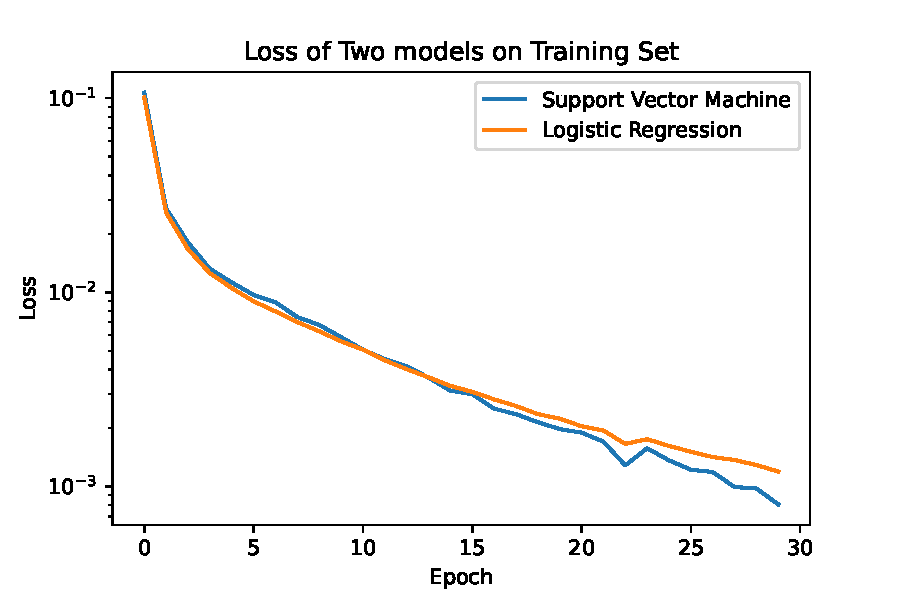
\includegraphics[width=0.6\textwidth]{Accuracy_with_epoch}
	\caption{Training loss of SVM and Logistic Regression model over 30 epochs.}
	\label{fig:acc_and_loss}
\end{figure}

\subsection*{Results for Two Optimisers}
I experimented with different momentum value for SGD optimiser. When $momentum = 0$, original SGD optimiser is adopted. Results are shown below in Figure \ref{fig:momentum}.

We can find from the figure \ref{fig:momentum} that when value of momentum increase, the loss become more unstable though still decreasing. From the equation of SGD-momentum we can know that when value of momentum increase, in gradient, more information from previous samples are kept. Under some cases this is helpful for reducing training loss, but may negatively influence the stability of loss when momentum is large. 

%Specially, when momentum is 1, the training process is only utilising the gradient from 

\begin{figure}[]
	\centering
	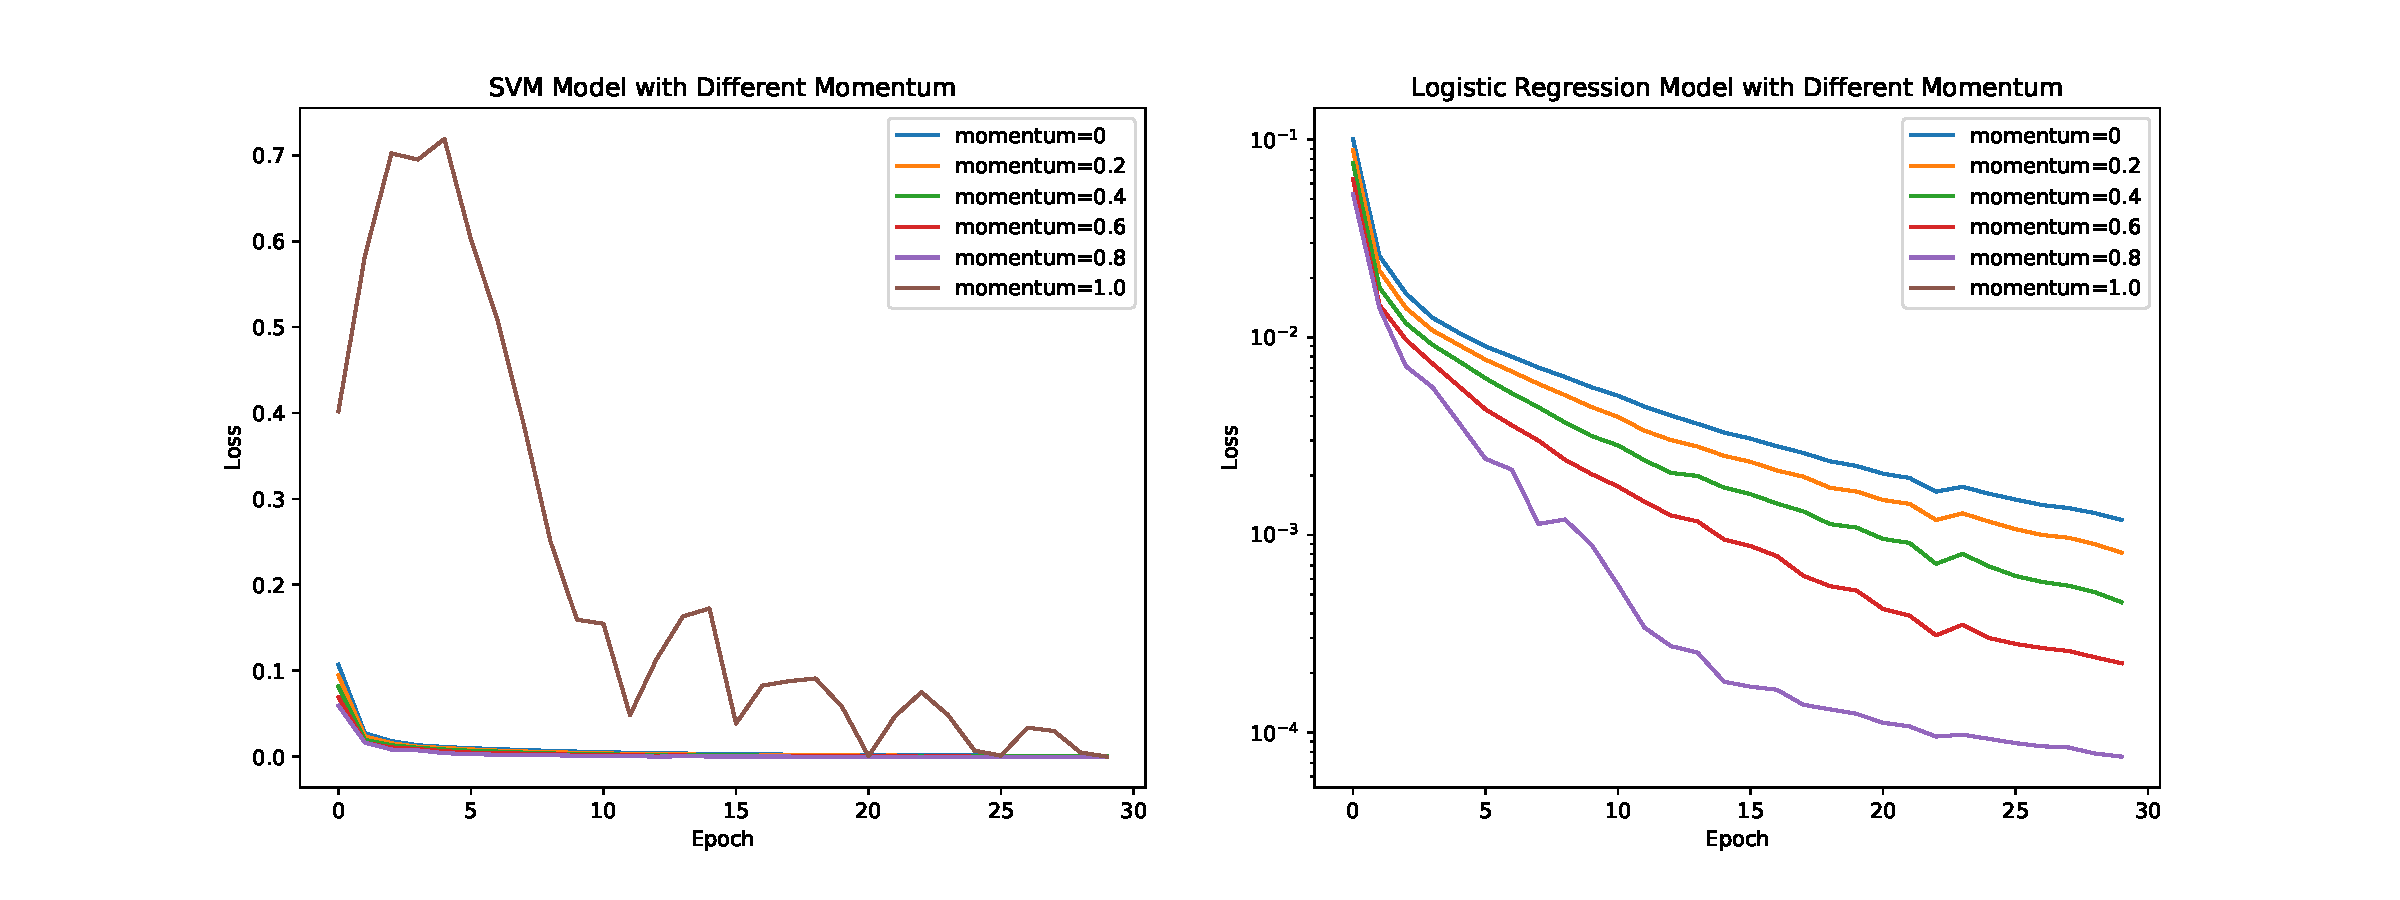
\includegraphics[width=\textwidth]{Two_Model_with_Different_Momentum.pdf}
	\caption{Different momentum value for SVM and Logistic Regression model under training set. In this experiment, step size was fixed to 0.1 for both models}
	\label{fig:momentum}
\end{figure}

\subsection*{Training with Different Step Size}
I experimented with step size on log scale, i.e., $lr \in \{10^{-4}, 10^{-3},10^{-2},0.1 ,1, 10\}$. The results are shown in Figure \ref{fig:step_size}.

\begin{figure}[h!]
	\centering
	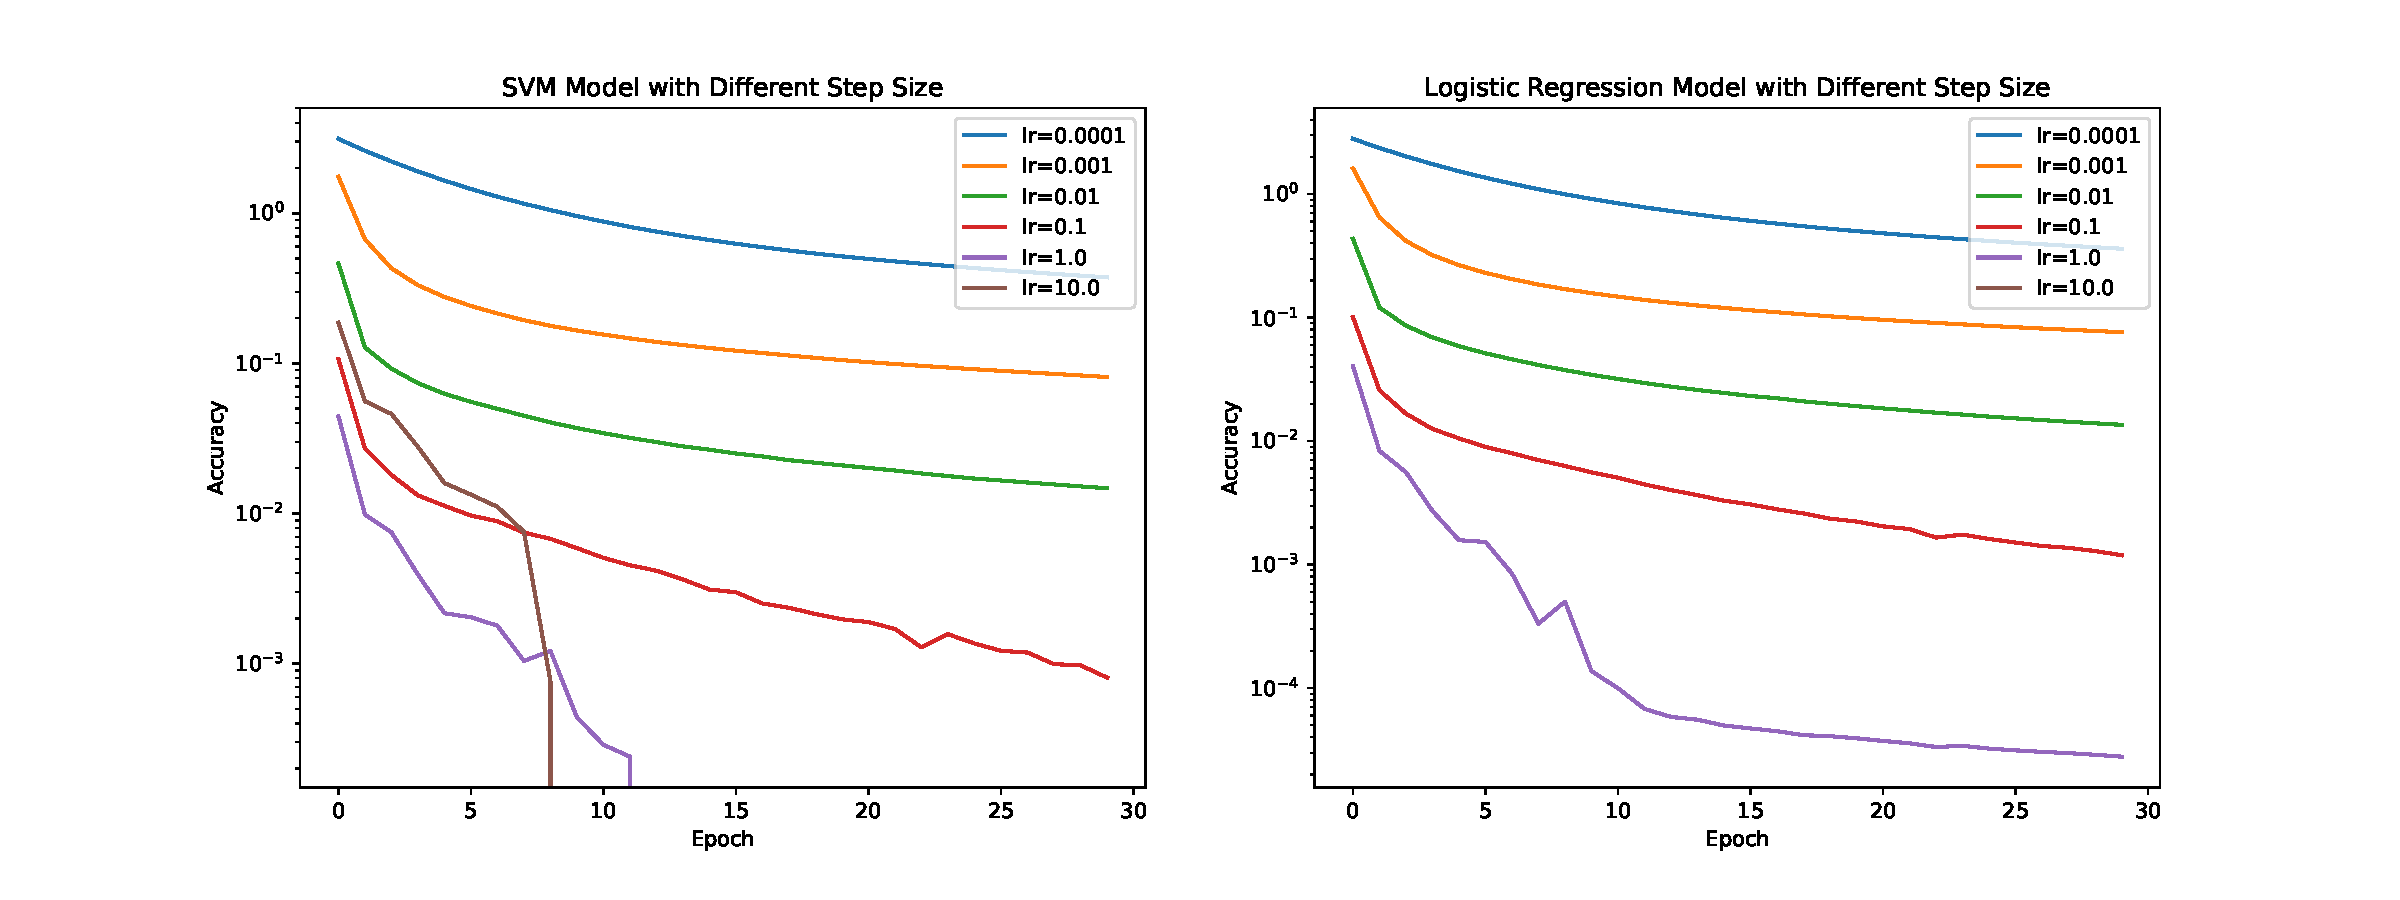
\includegraphics[width=\textwidth]{Two_Models_with_Different_Step_Size}
	\caption{Train model with different step size.}
	\label{fig:step_size}
\end{figure}

Generally speaking, a larger step size helps model to converge faster. However, when step size is too large, the loss may explode and result in ``nan'' in Python. This is observed when step size is 10 for logistic model.

Besides, a large step size may add to instability during training. As shown in the figure \ref{fig:step_size}, with a large step size, the curve of loss may not be as smooth as the loss curve with smaller step size.

\end{document}



